
Niniejszy rozdział ma na celu przedstawienie testów aplikacji oraz korzystania z jej. Zostały w nim umieszczone przykładowe sposoby użycia funkcji dostępnych w aplikacji mobilnej.



\section{Zarządzanie kontem}{
	


Użytkownik w celu korzystania z aplikacji musi być zalogowany. Pierwsze uruchomienie aplikacji skutkuje uruchomieniem ekranu logowania. W przypadku gdy użytkownik wcześniej zalogował się, a token dostępu nie wygasł, wówczas dostępny jest ekran główny aplikacji. Ze względu na asynchroniczną komunikację z serwerem poprzez zapytania HTTP, użytkownik w trakcie oczekiwania na odpowiedź ma przedstawiony ekran ładowania. W przypadku otrzymania błędu lub wykonania zabronionej operacji na serwerze, użytkownik otrzyma powiadomienie na dole ekranu.

\begin{figure}[h]
	\centering
	\subfloat[Ekran logowania.]{\label{odnosnik}
		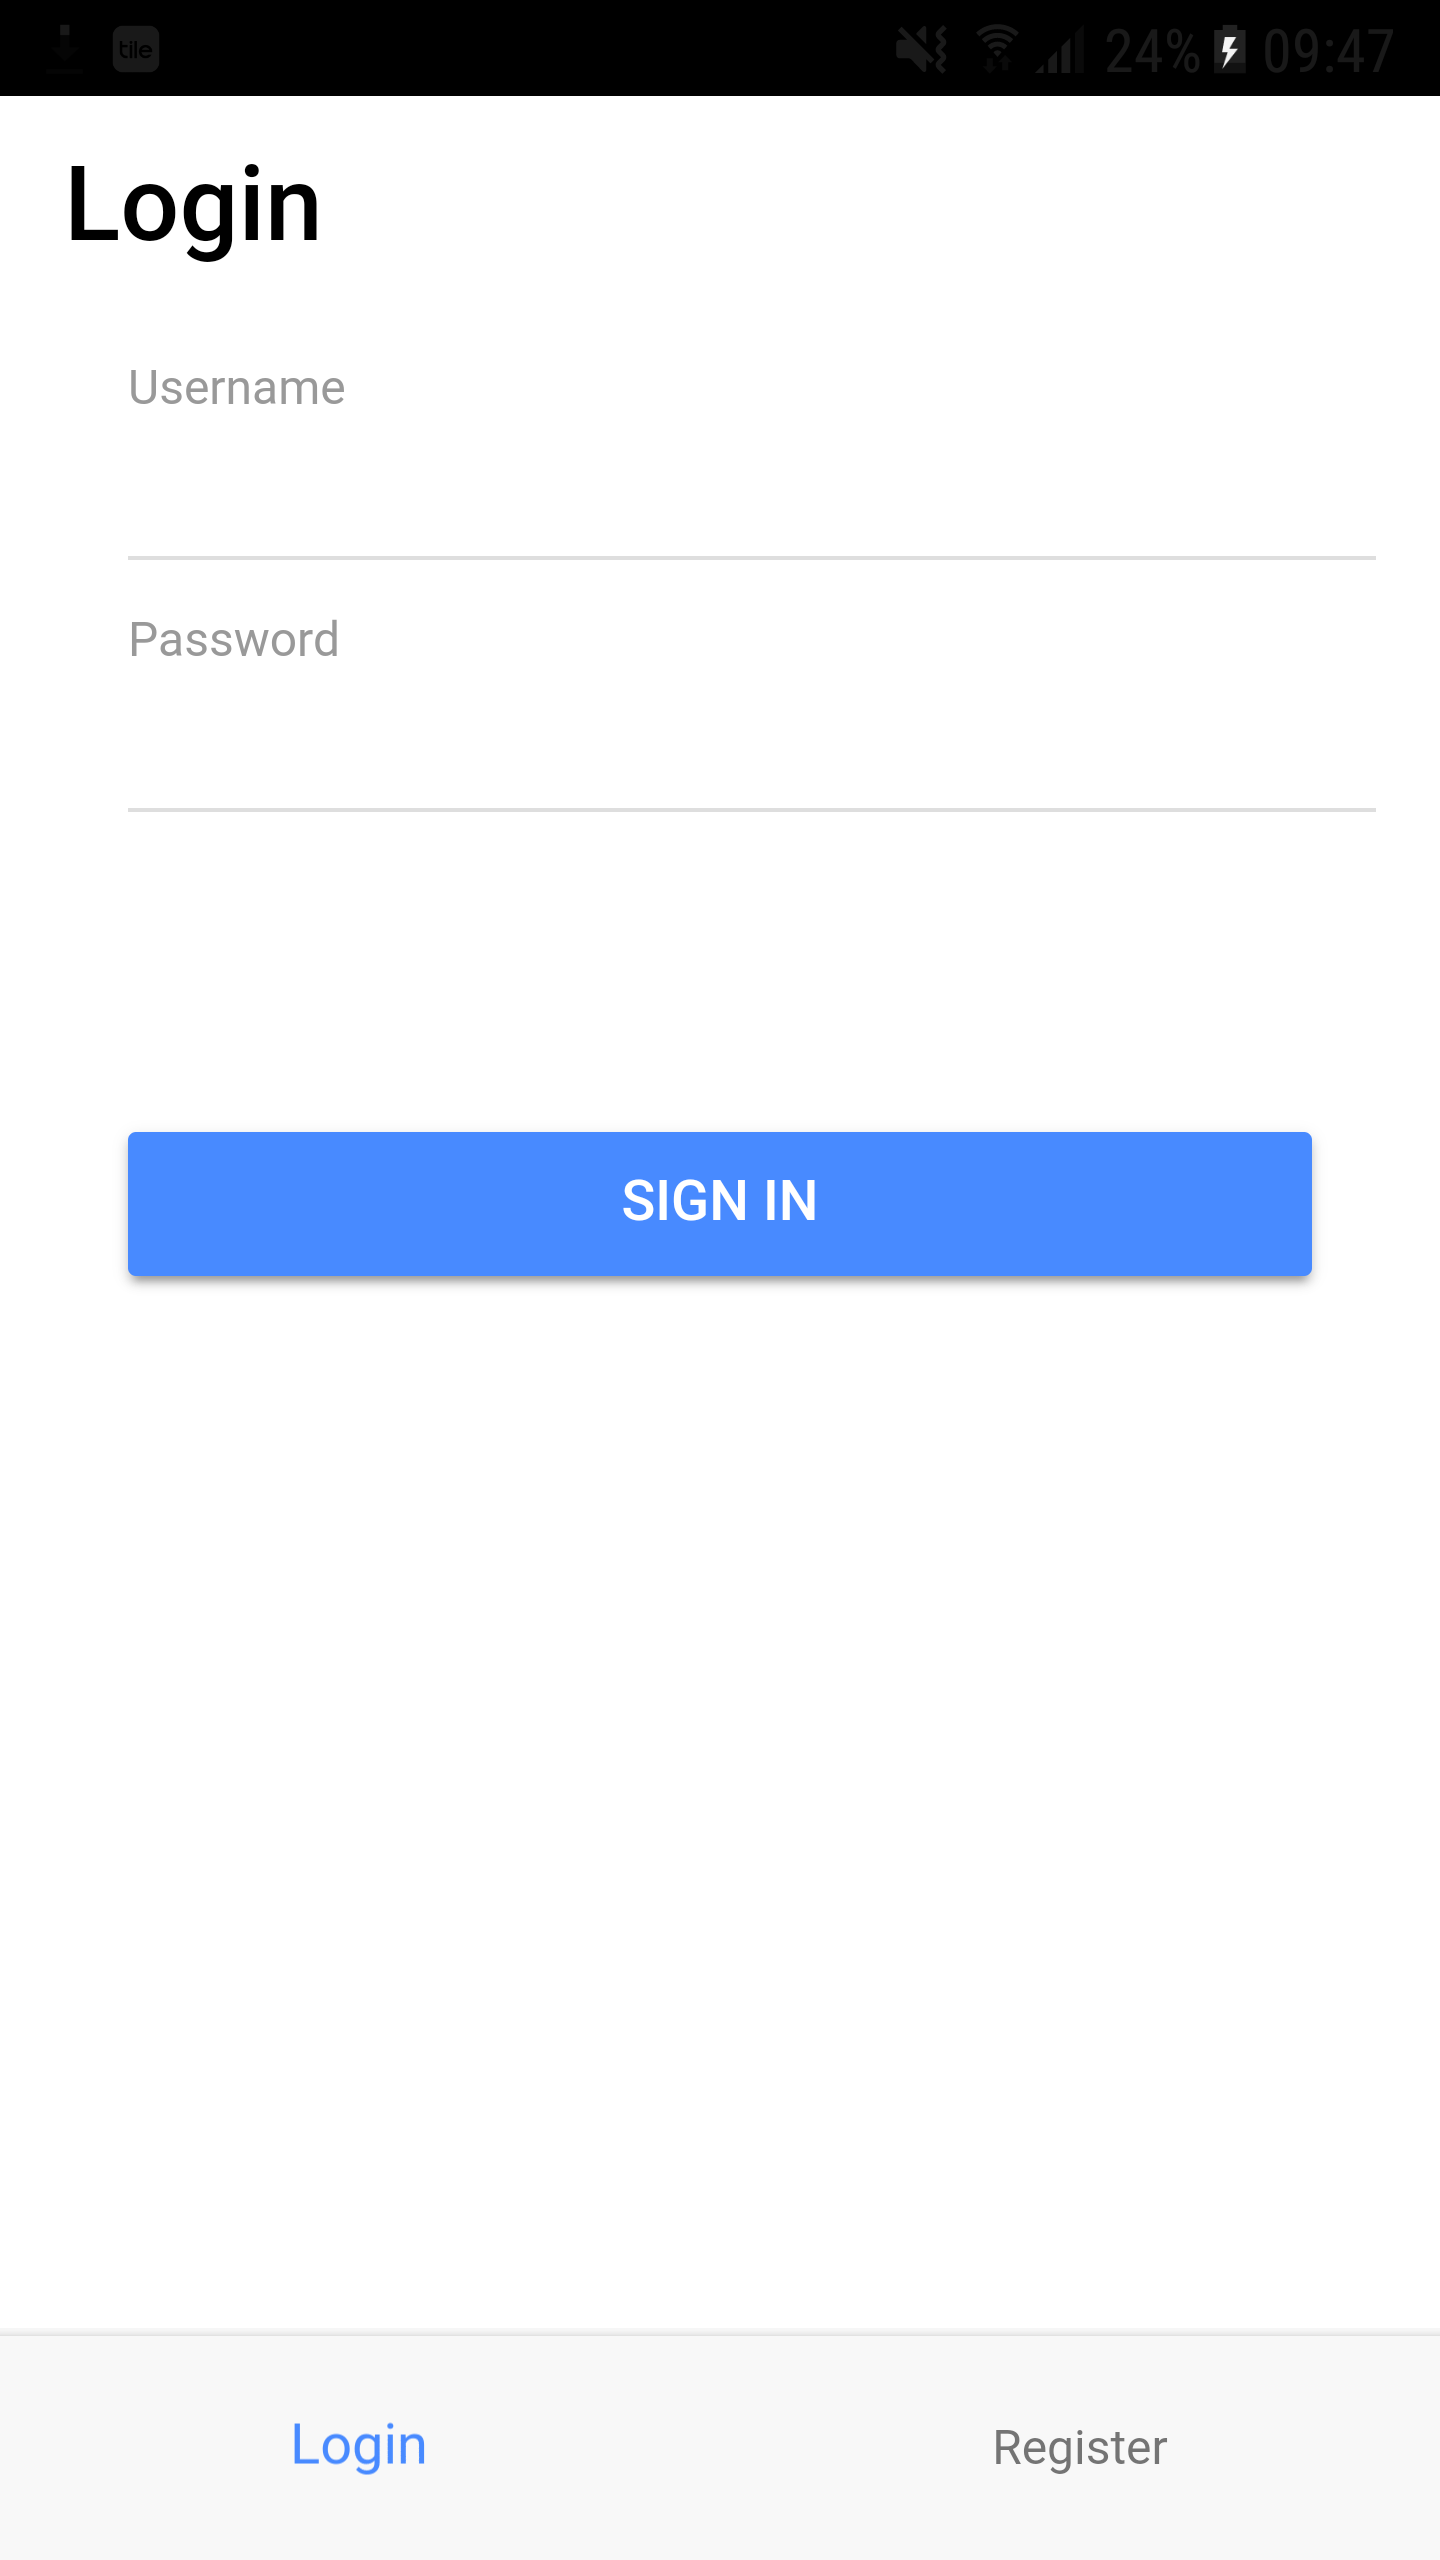
\includegraphics[width=0.4\textwidth]{images/login_page}}
	\quad
	\subfloat[Ekran rejestracji.]{\label{odnosnik}
		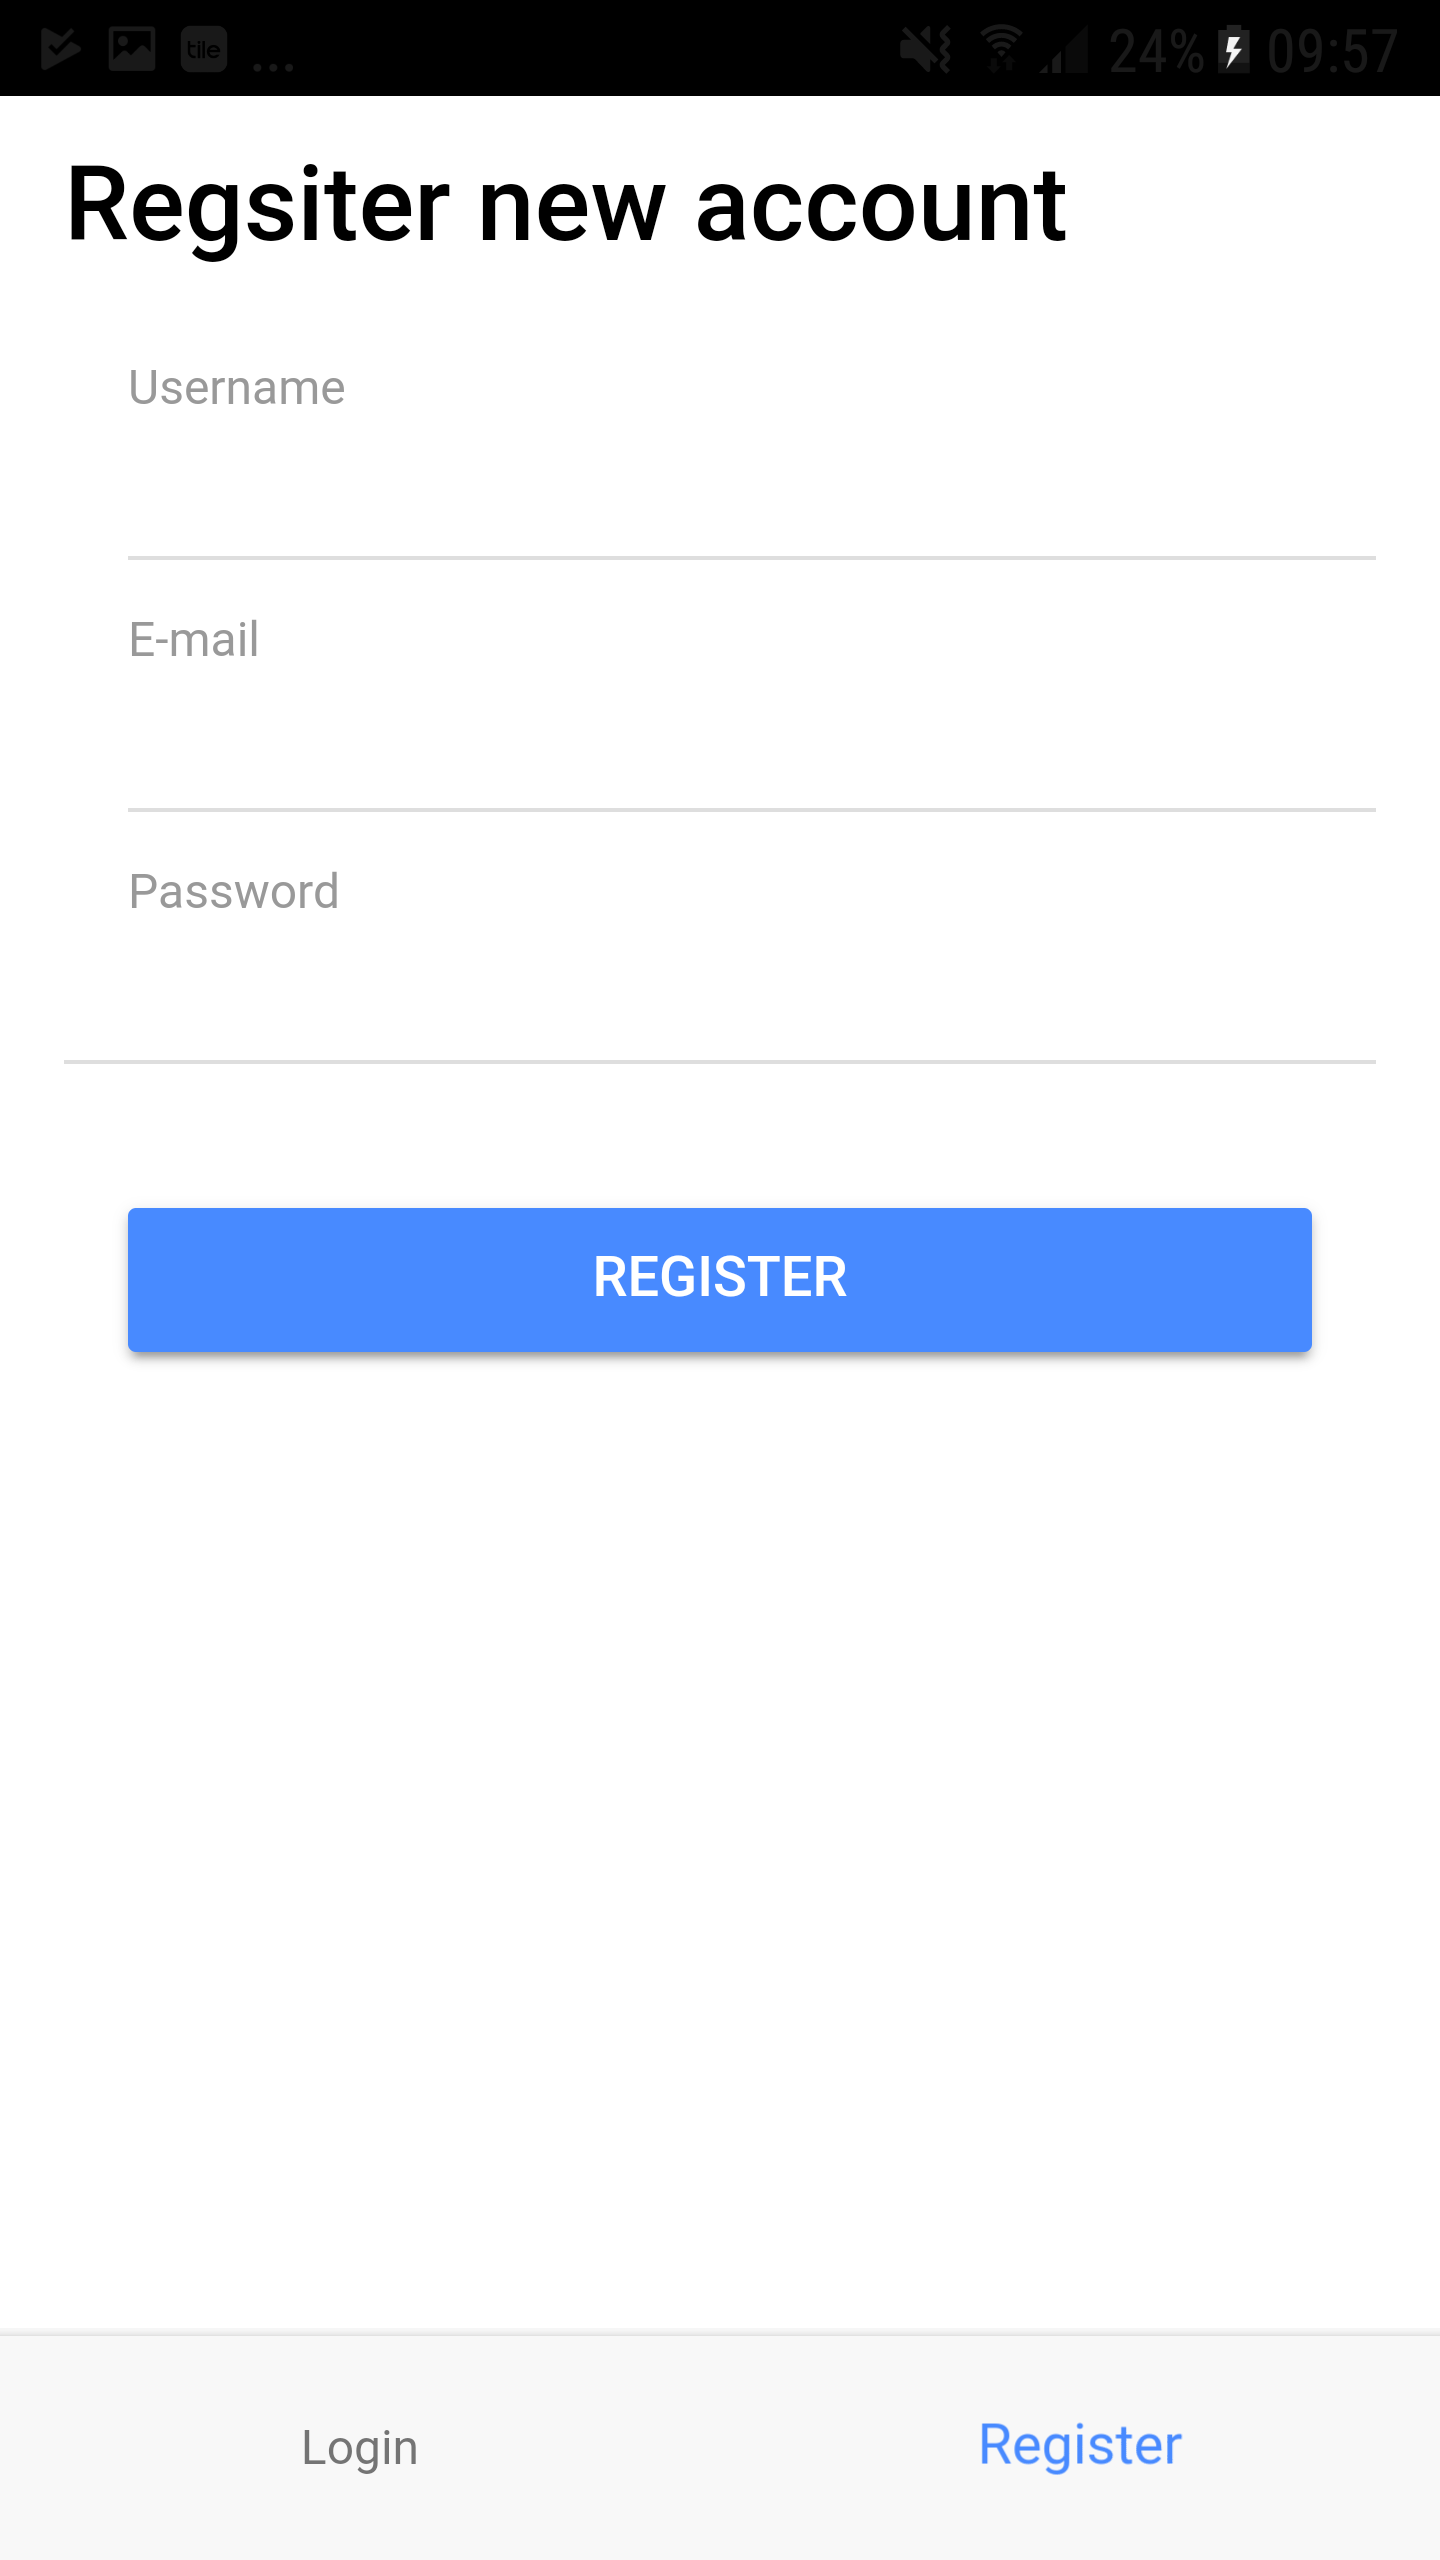
\includegraphics[width=0.4\textwidth]{images/register_page}}
	\caption{Ekrany logowania i rejestracji}
	\label{fig:registerpage}
\end{figure}

W przypadku gdy użytkownik nie posiada konta, zalecane jest skorzystanie z zakładki "Rejestracja". Umożliwia ona wpisanie podstawowych informacji niezbędnych do założenia konta. Zostały nałożone również restrykcje dotyczące polityki bezpieczeństwa konta. W związku z tym podczas rejestracji użytkownik jest proszony o:
\begin{itemize}[noitemsep]
	\item podanie adresu e-mail,
	\item podanie unikalnej nazwy użytkownika,
	\item ustawienie hasła zawierającego co najmniej trzy znaki.
\end{itemize} 
}
\newpage
\section{Zarządzanie zdjęciami}{

Pomyślna rejestracja oraz zalogowanie użytkownika przenoszą go do ekranu głównego aplikacji.Pierwszy widok zawiera instrukcje zachęcające do zrobienia nowego zdjęcia lub wybrania go z galerii. Ponadto na ekranie dostępne są dodatkowe zakładki - "History" oraz "Contact". Użytkownik ma możliwość wylogowania się dzięki przyciskowi "Logout" znajdującemu się w prawym górnym rogu ekranu. Pierwszy ekran umożliwia przesłanie zdjęcia do serwera aplikacji w celu dalszego przetwarzania. Aby zrobić zdjęcie, należy wybrać przycisk "TAKE PHOTO", który uruchomi kamerę. Aplikacja będzie oczekiwała do momentu przekazania zdjęcia z urządzenia mobilnego. W przypadku wybrania przycisku "SELECT FROM GALLERY", aplikacja uruchomi systemowy eksplorator zdjęć. Wybór jednego z nich będzie równoznaczny dla aplikacji ze zrobieniem zdjęcia z aparatu. Aplikacja po wybraniu obrazu wyświetli go na ekranie głównym oraz udostępni przyciski "Send" oraz "Remove". Wybranie przycisku "Send" prześle zdjęcie na serwer. W przypadku przycisku "Remove" przesyłanie zostanie anulowane.

	
\begin{figure}[h]
	\centering
	\subfloat[Główny widok aplikacji]{\label{odnosnik}
		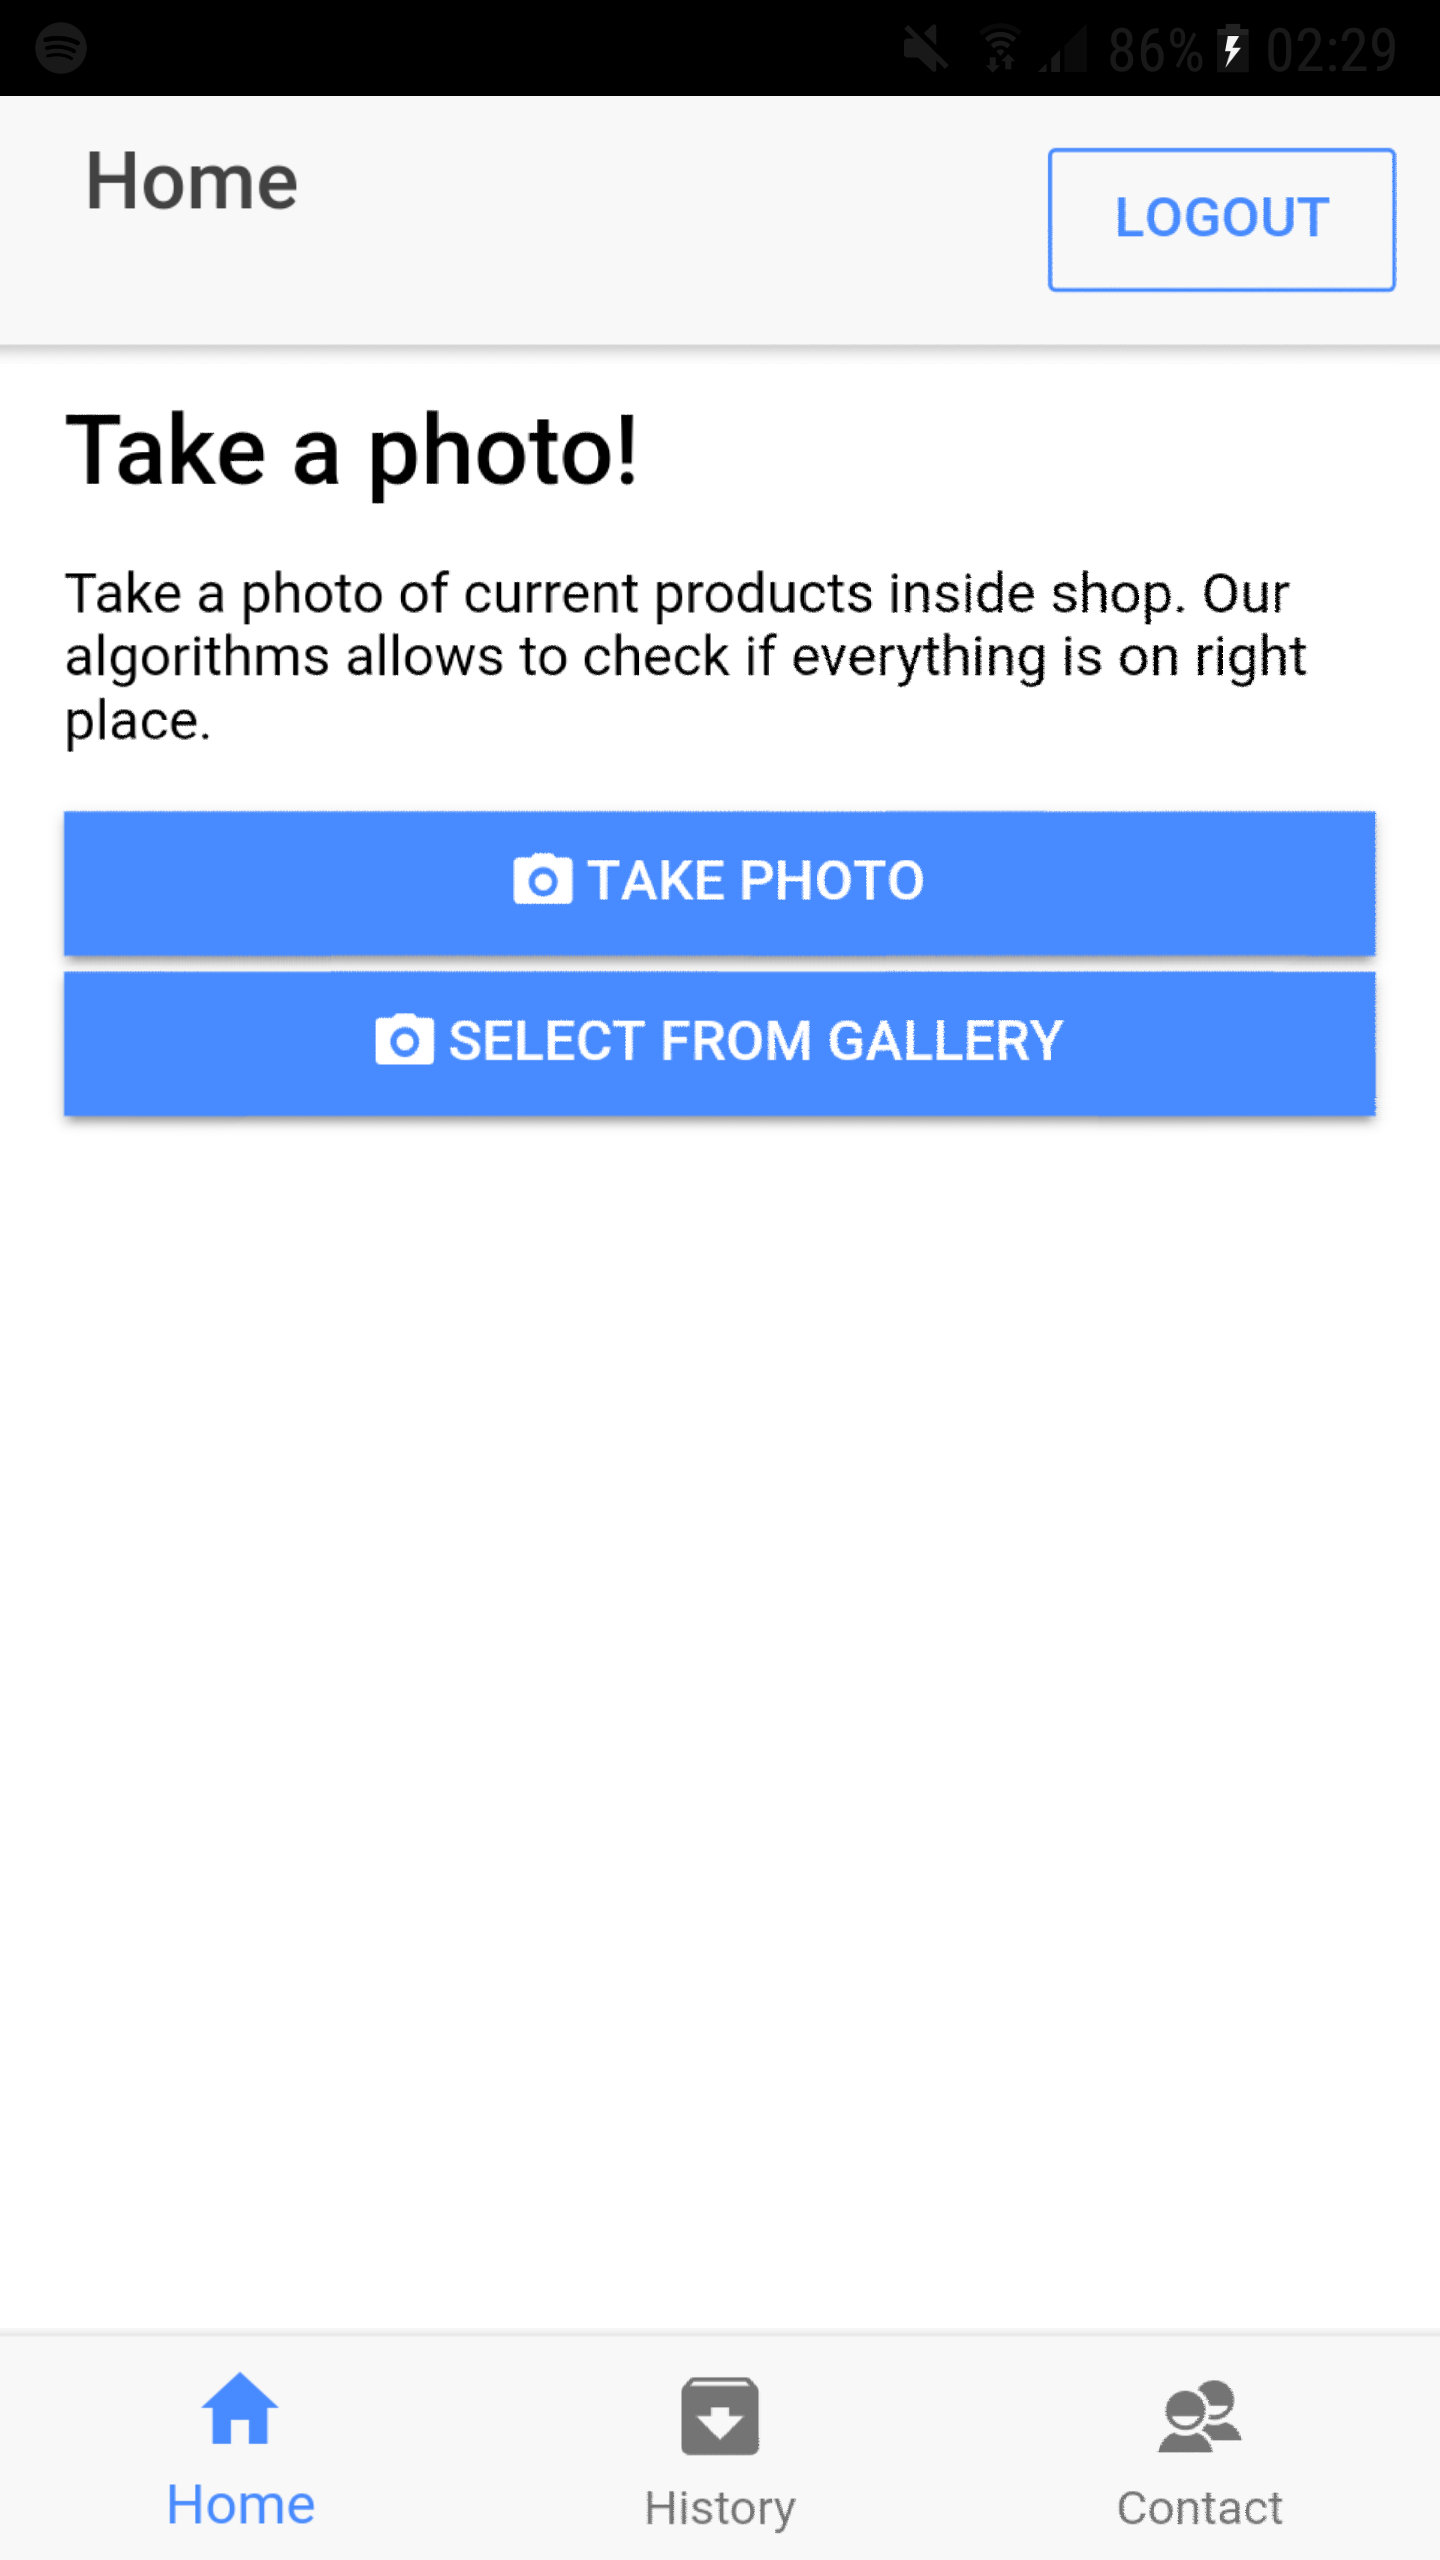
\includegraphics[width=0.4\textwidth]{images/home_page}}
	\quad
	\subfloat[Widok wysłania zdjęcia]{\label{odnosnik}
		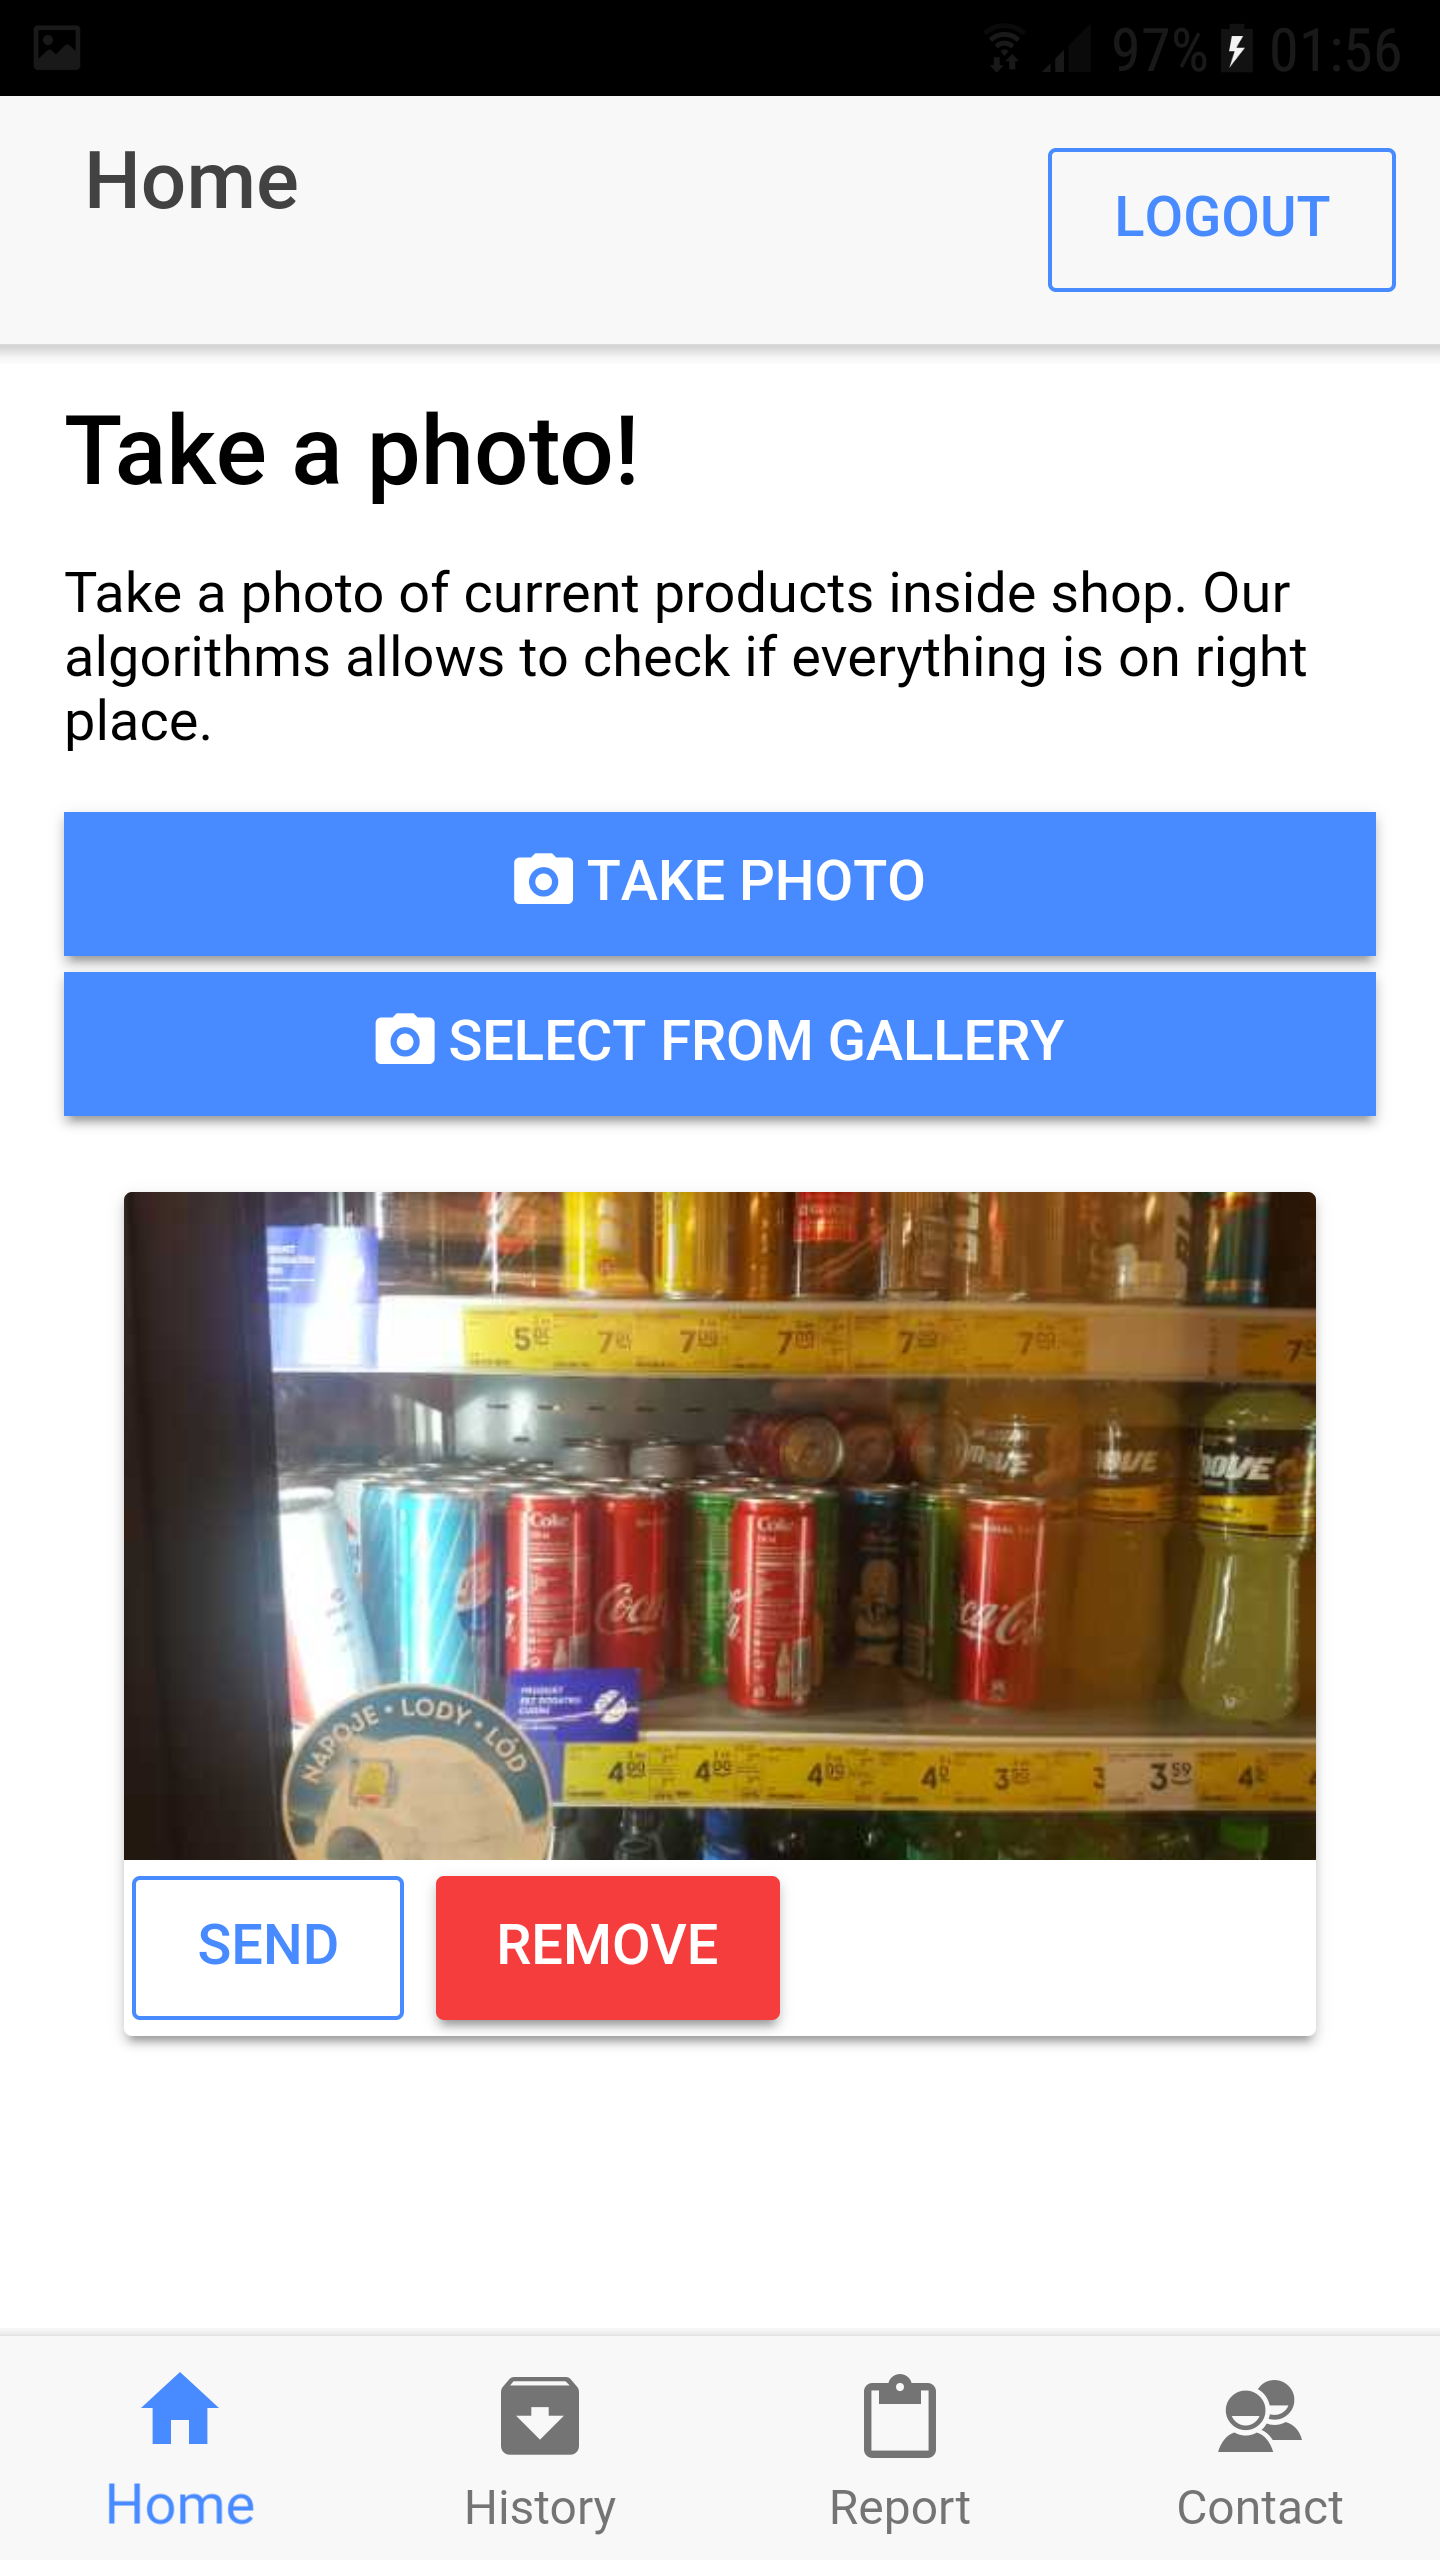
\includegraphics[width=0.4\textwidth]{images/upload_page}}
	\caption{Ekran domowy oraz wysłania zdjęcia.}
	\label{fig:uploadView}
\end{figure}

Użytkownik w celu poddania zdjęcia analizie może wybrać zdjęcie z galerii lub stworzyć je przy użyciu aparatu z ekranu głównego. Udostępnienie zdjęcia na serwer spowoduje uruchomienie algorytmów detekcji przedmiotów oraz przetwarzania ontologii. W momencie oczekiwania na dokonanie obliczeń użytkownik czeka na odpowiedź serwera na ekranie ładowania. Po zakończeniu przetwarzania danych ekran wyświetli okno szczegółów analizy. Dzięki niemu użytkownik może dowiedzieć się wyników klasyfikacji przedmiotów oraz przetwarzania reguł semantycznych. Ekran został podzielony na trzy sekcje - zdjęcie (Image), typy(Types) oraz wartości (values). Użytkownik w zależności od wybranej sekcji otrzymają różnego typu dane. Zakładka zdjęcia (Image) zawiera aktualnie przetworzone zdjęcie wraz z zaznaczeniem przedmiotów na nim oraz ich pozycje. Przejście do zakładki typów (Types) spowoduje wyświetlenie zbiorów typów dla każdego sklasyfikowanego przedmiotu. Przetworzenie ontologii dostarcza informacji o relacjach zachodzących miedzy indywiduami. Dane te użytkownik może znaleźć w zakładce wartości (Values)  Aby wyjść z ekranu należy skorzystać z pola x, które znajduje się w prawym górnym rogu ekranu.

	
\begin{figure}[ht]
	\centering
	\subfloat[Szczegóły wnioskowania.]{\label{odnosnik}
		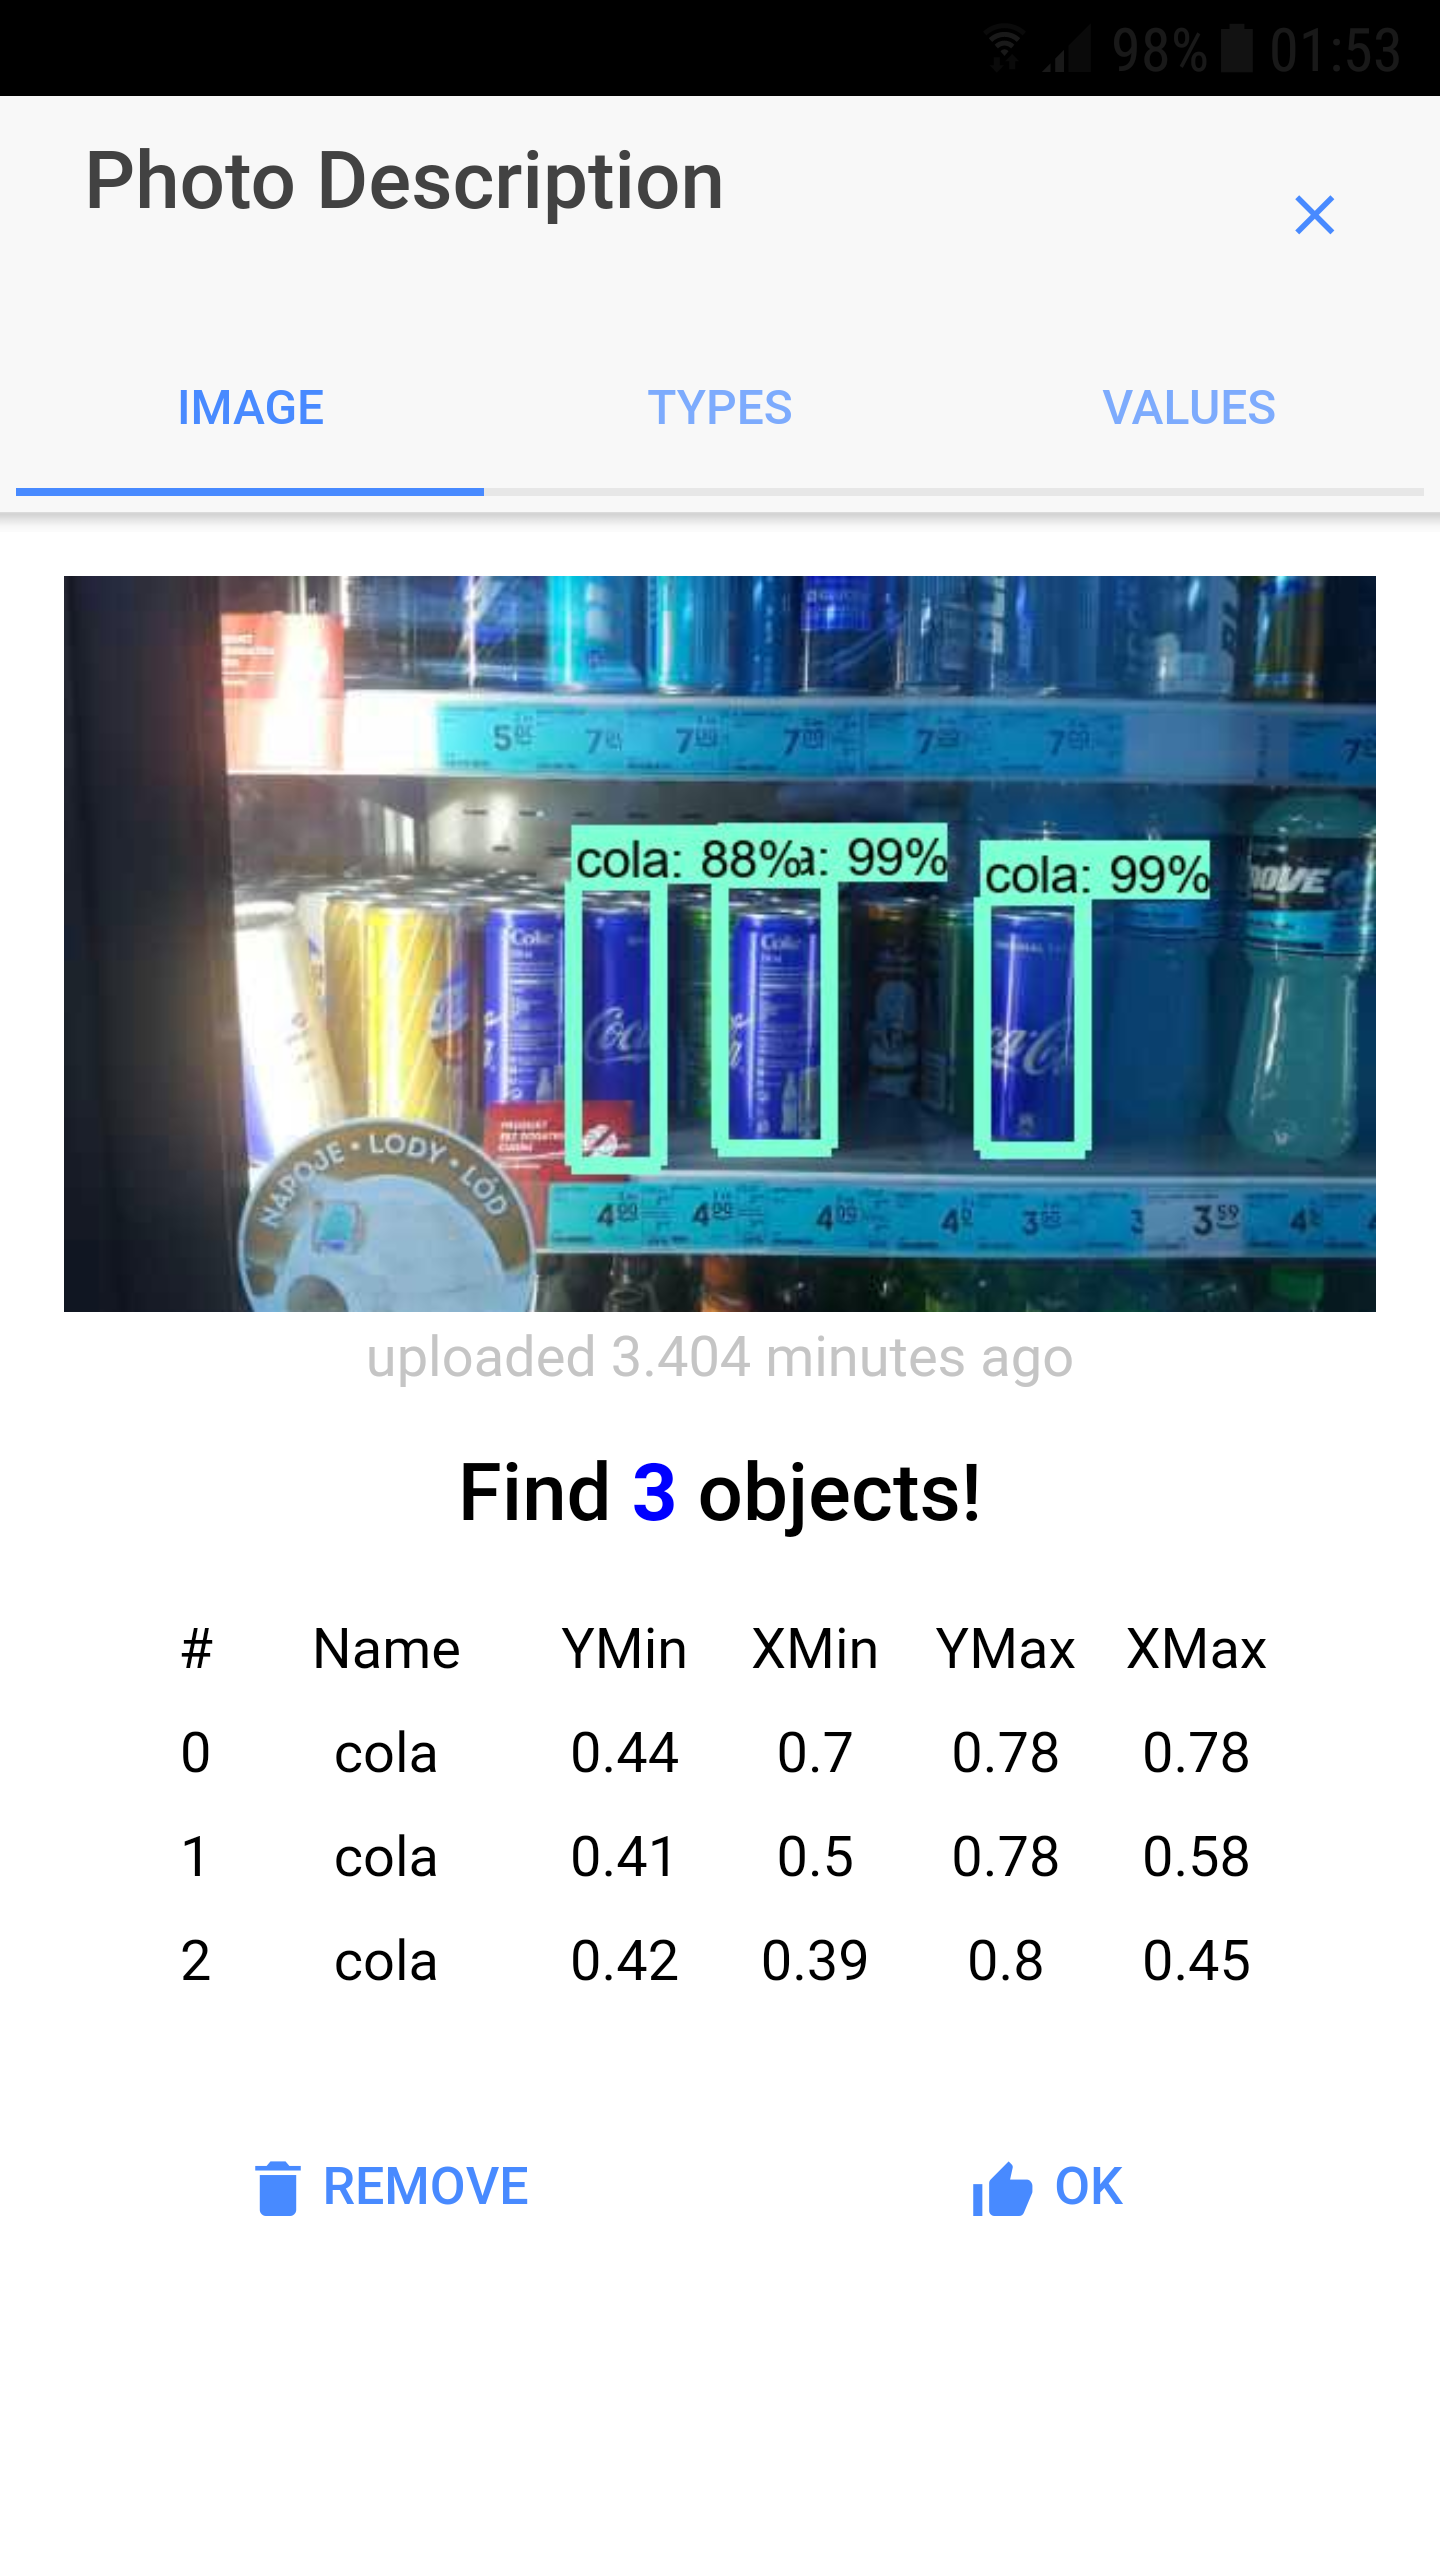
\includegraphics[width=0.4\textwidth]{images/details}}
	\quad
	\subfloat[Szczegóły wnioskowania - otrzymane klasy.]{\label{odnosnik}
		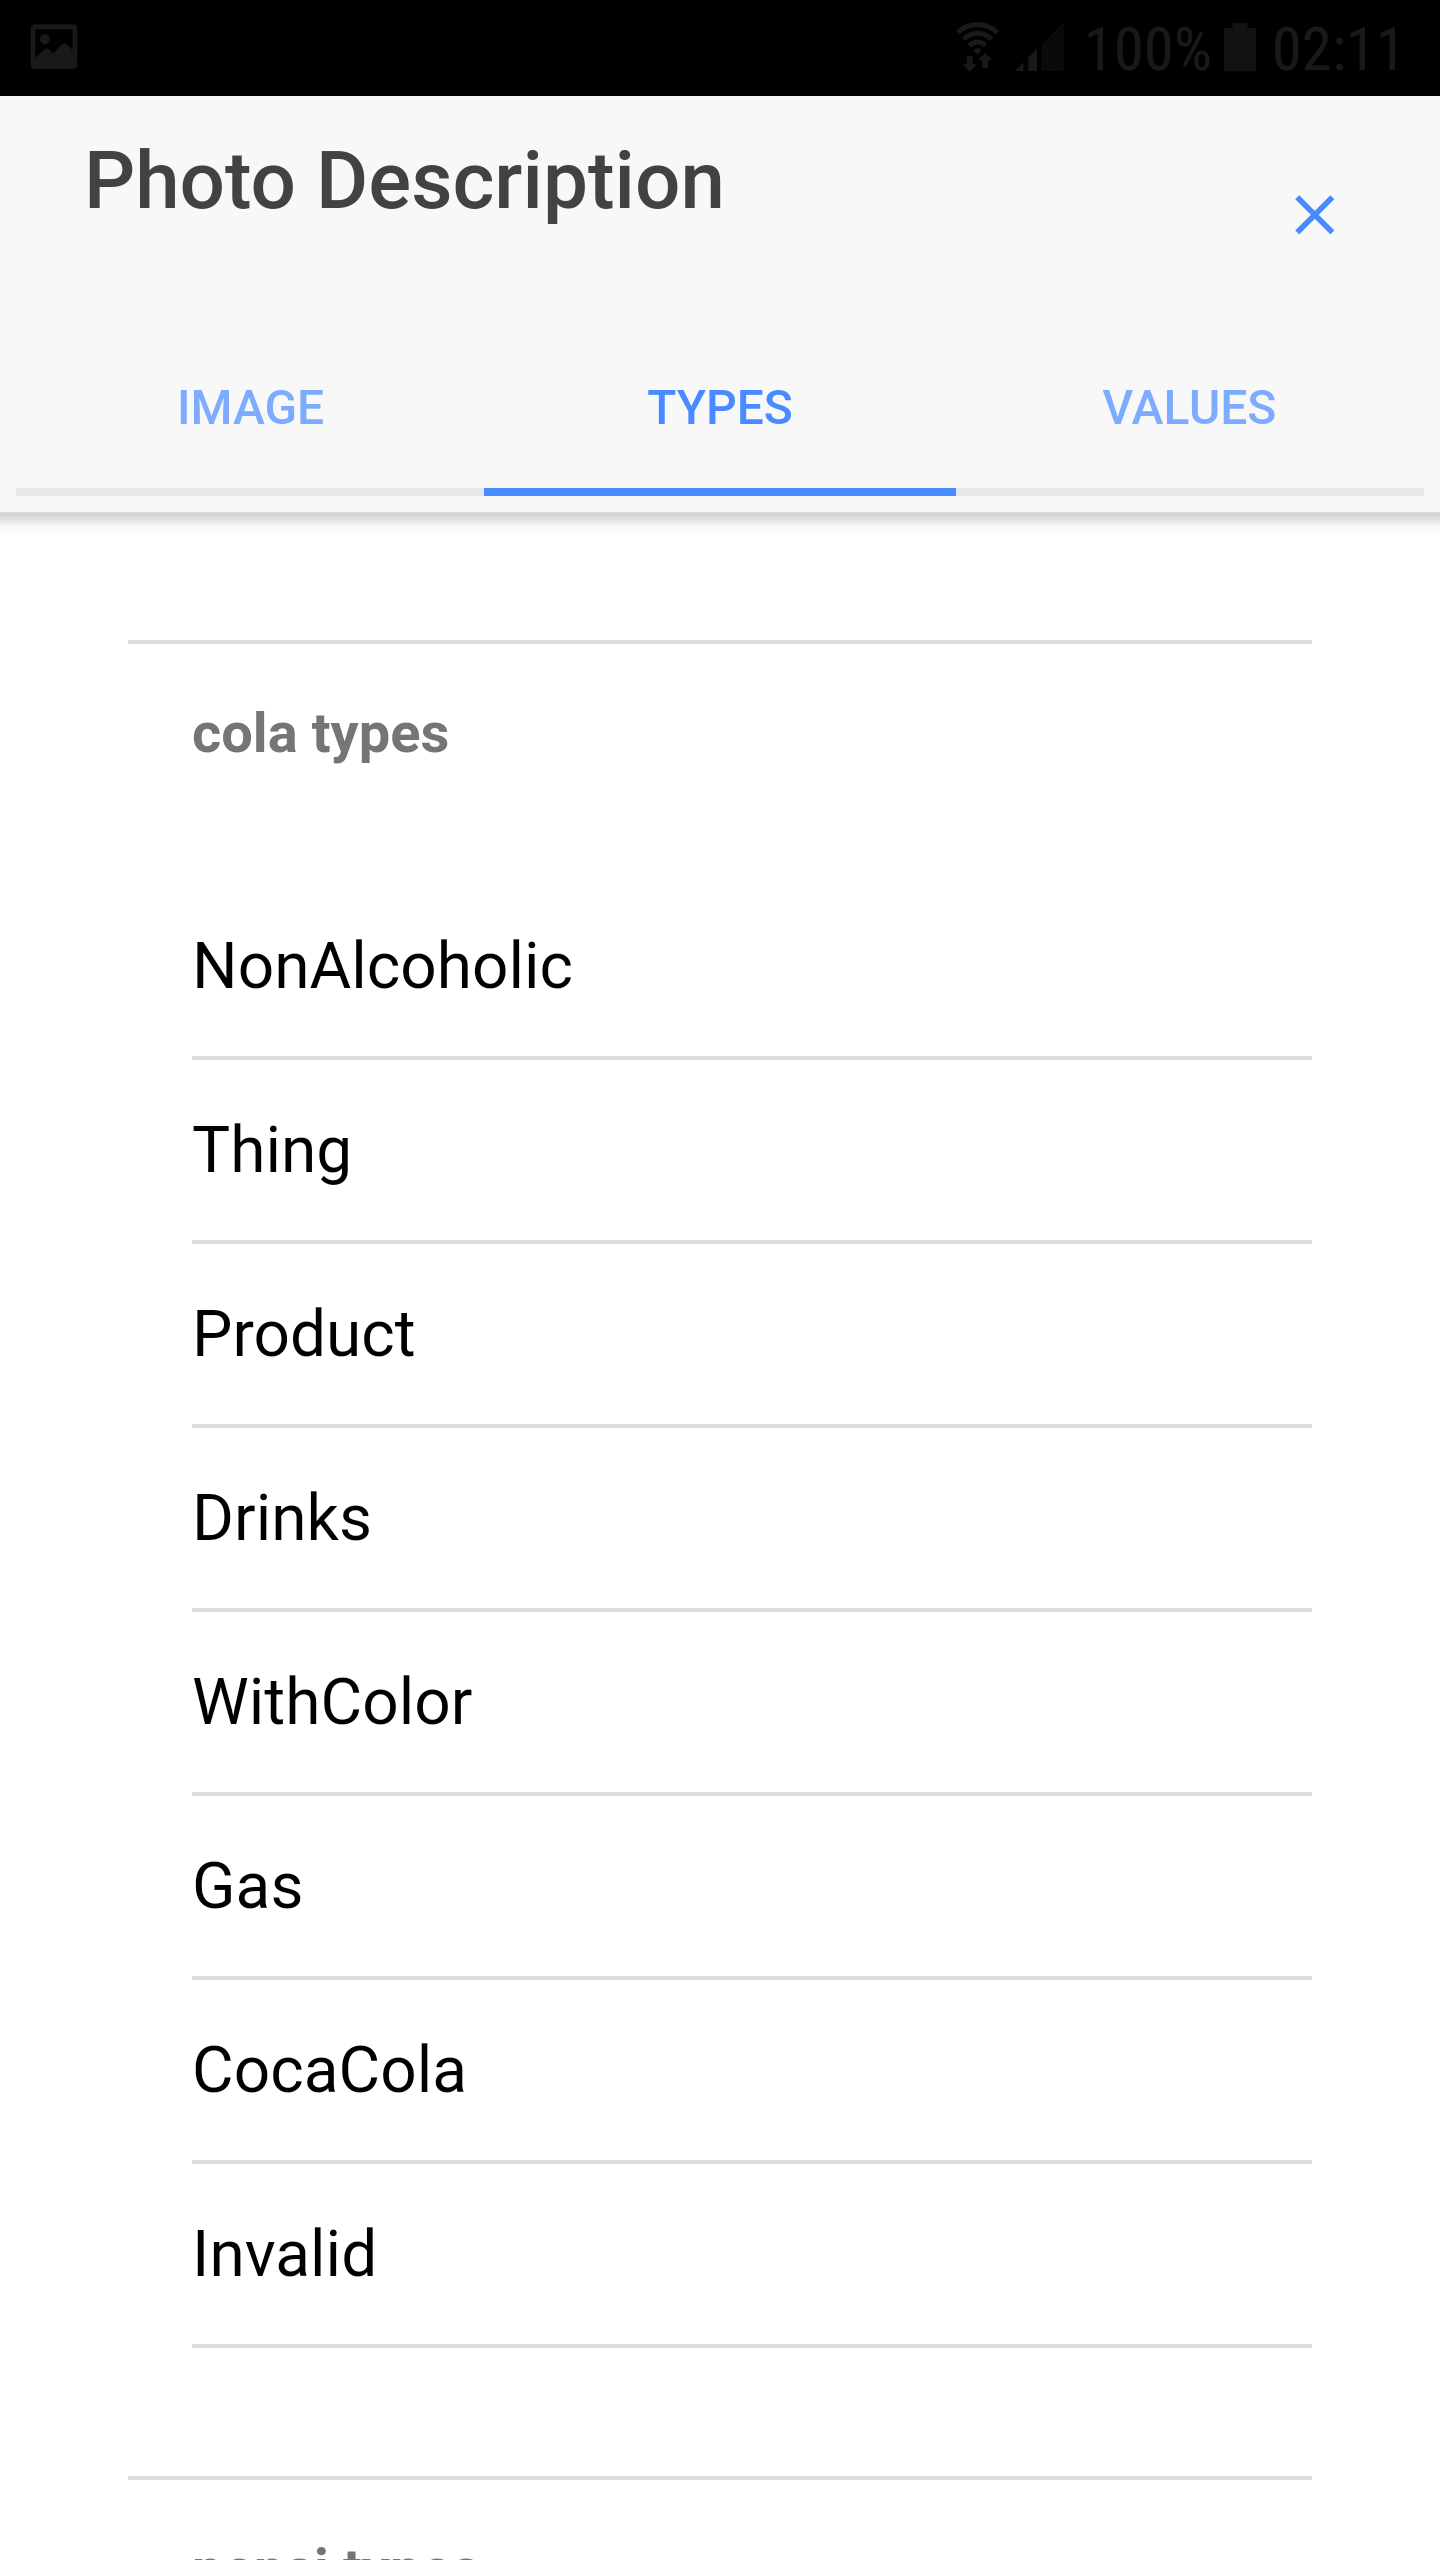
\includegraphics[width=0.4\textwidth]{images/types}}
	\caption{Ekran szczegółów analizowanego zdjęcia.}
	\label{fig:uploadView}
\end{figure}

Użytkownik może wrócić do wcześniej wykonanych zdjęć oraz ich wyników. W celu z menu głównego należy dotknać pole archiwum (History). Wybranie zakładki spowoduje wyświetlenie zbioru przesłanych zdjeć wraz z wynikami przetwarzania. Na samym dole zakładki znajduje się menu nawigacyjne zbioru zdjęć historycznych. Nawigację można wykorzystać aby przejść do kolejnej strony wyników, cofnięcie się lub odświeżenie danych. Na każdym ze zdjęć można dokonać operacji usunięcia poprzez kliknięcie przycisku "Remove" oraz otrzymać szczegóły zdjęcia poprzez wybranie "Check details". Ekran szczegółów analizy nie różni się od ekranu otrzymanego zaraz po przesłaniu zdjęcia na serwer. 

\begin{figure}[ht]
	\centering
	\subfloat[Szczegóły wnioskowania - wnioski.]{\label{odnosnik}
		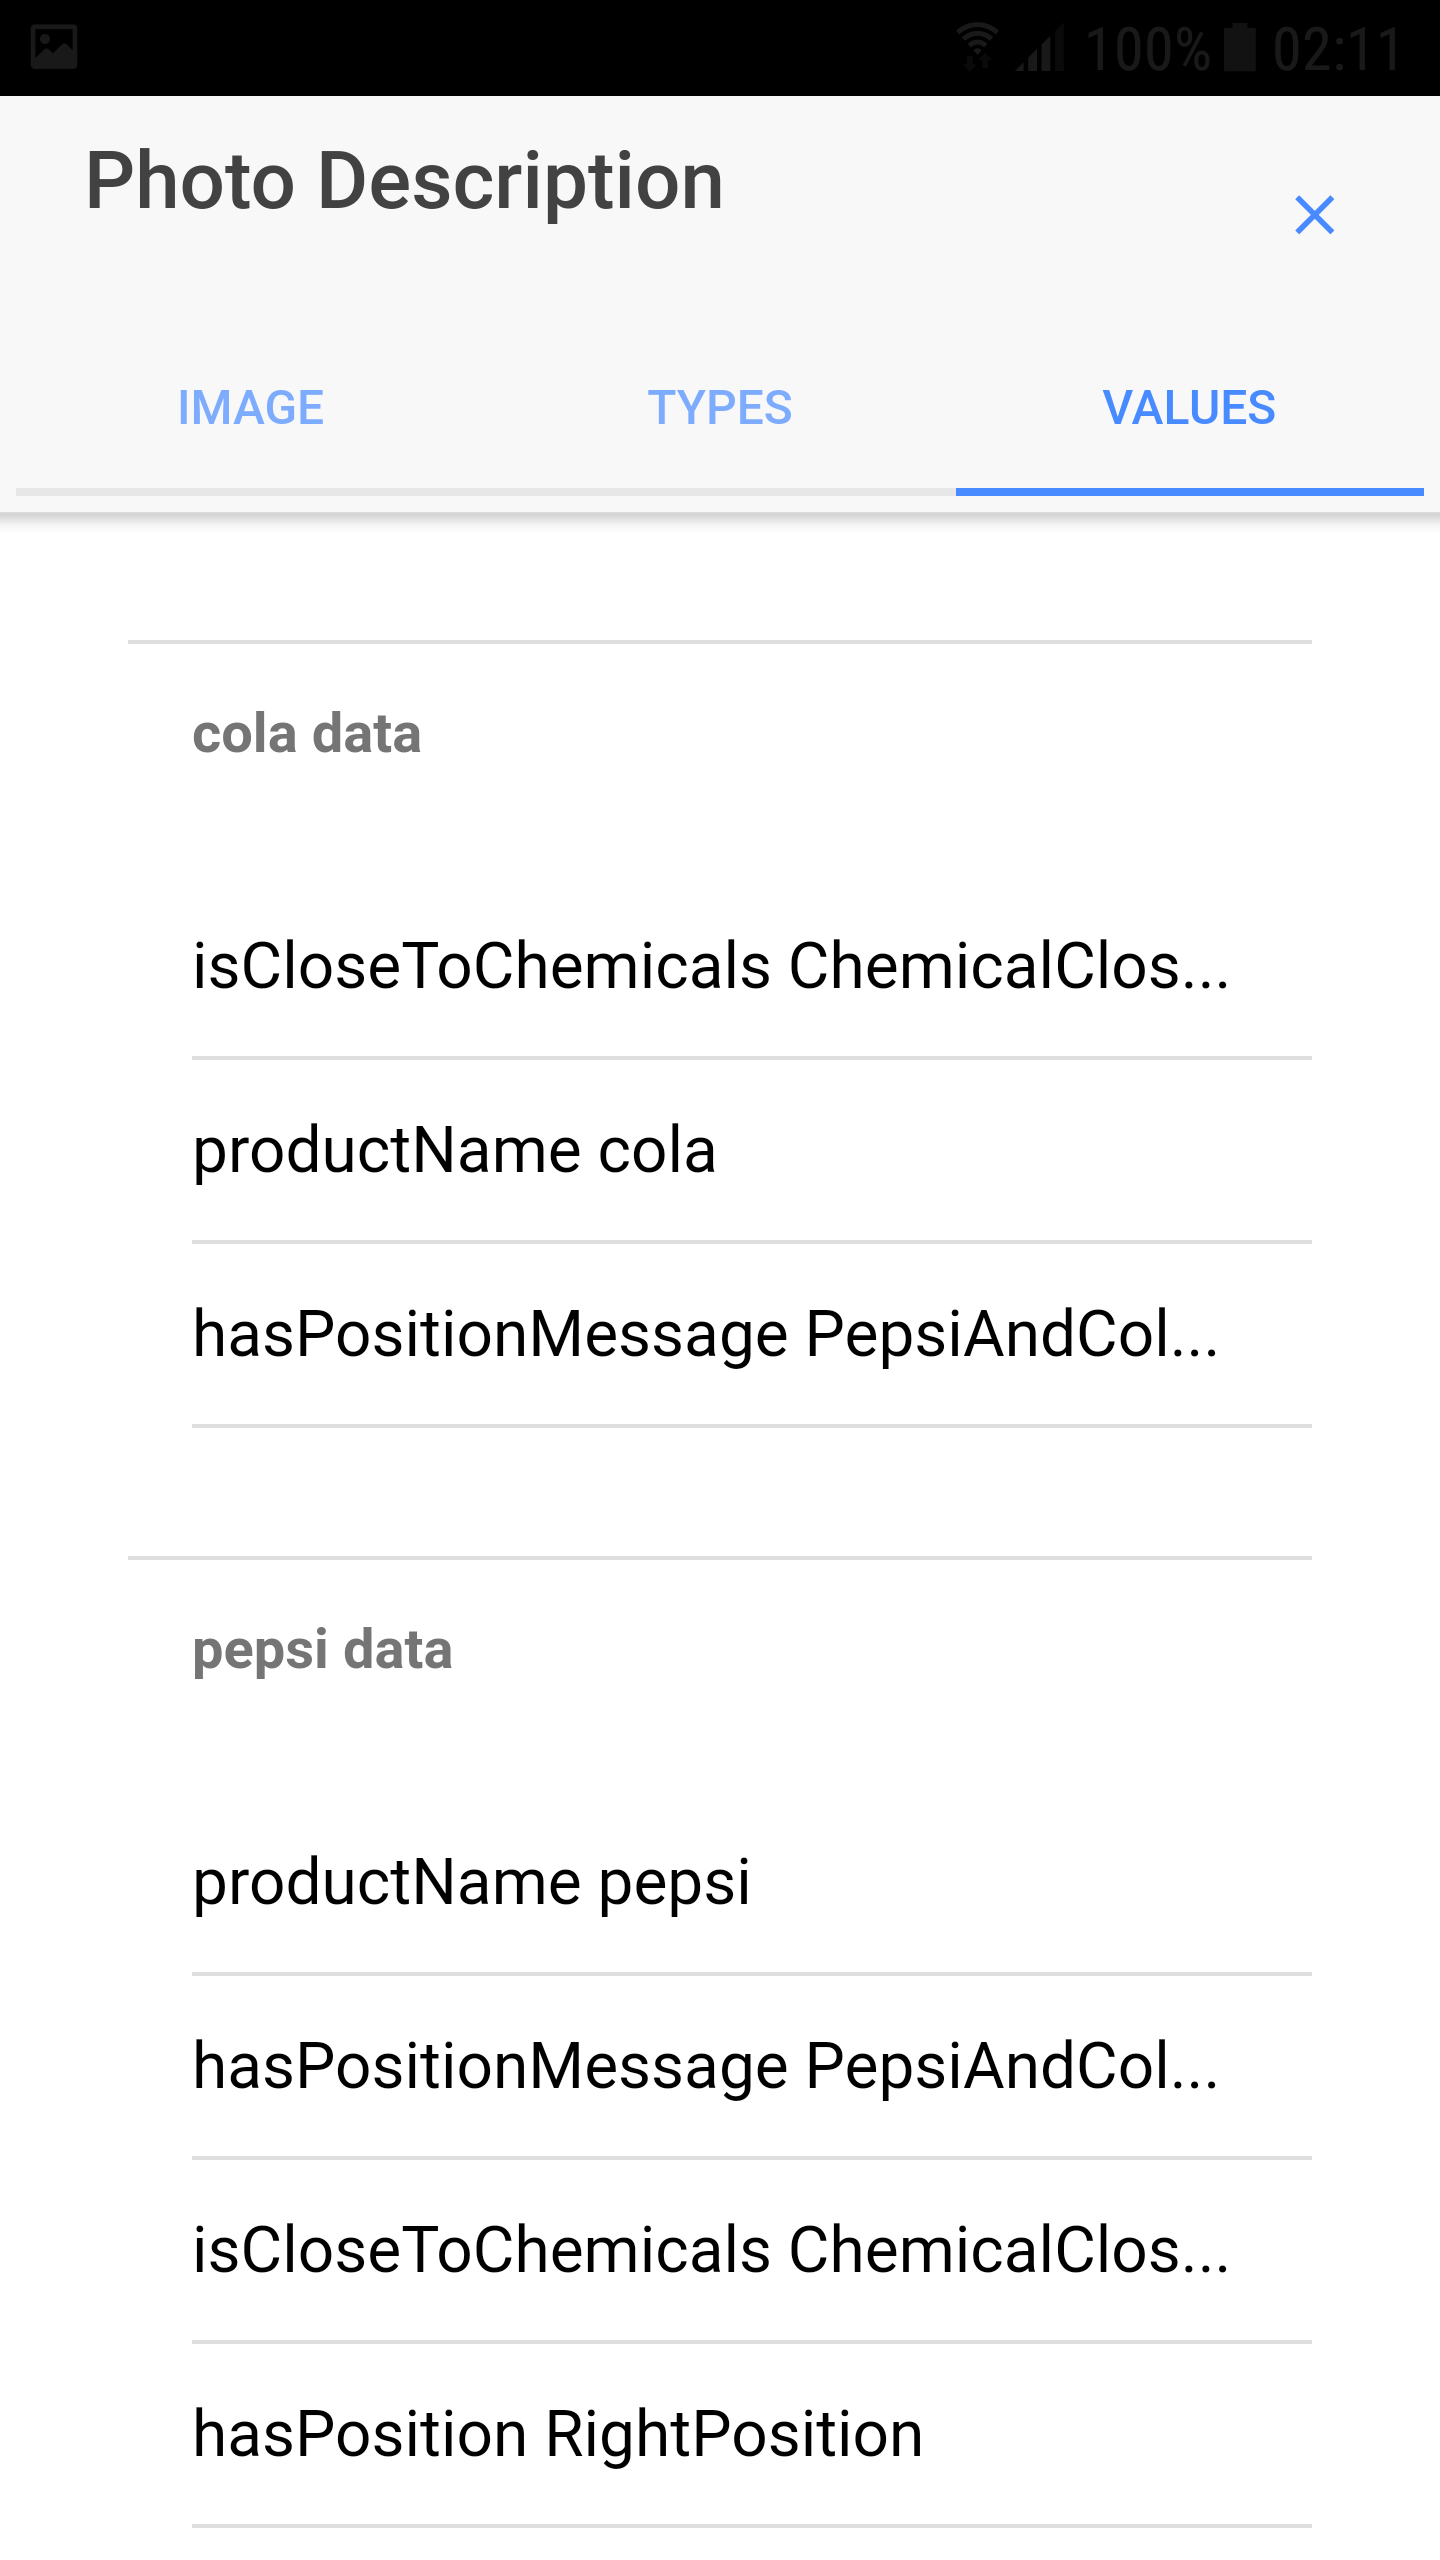
\includegraphics[width=0.4\textwidth]{images/values}}
	\quad
	\subfloat[Zbiór przeanalizowanych zdjęć.]{\label{odnosnik}
		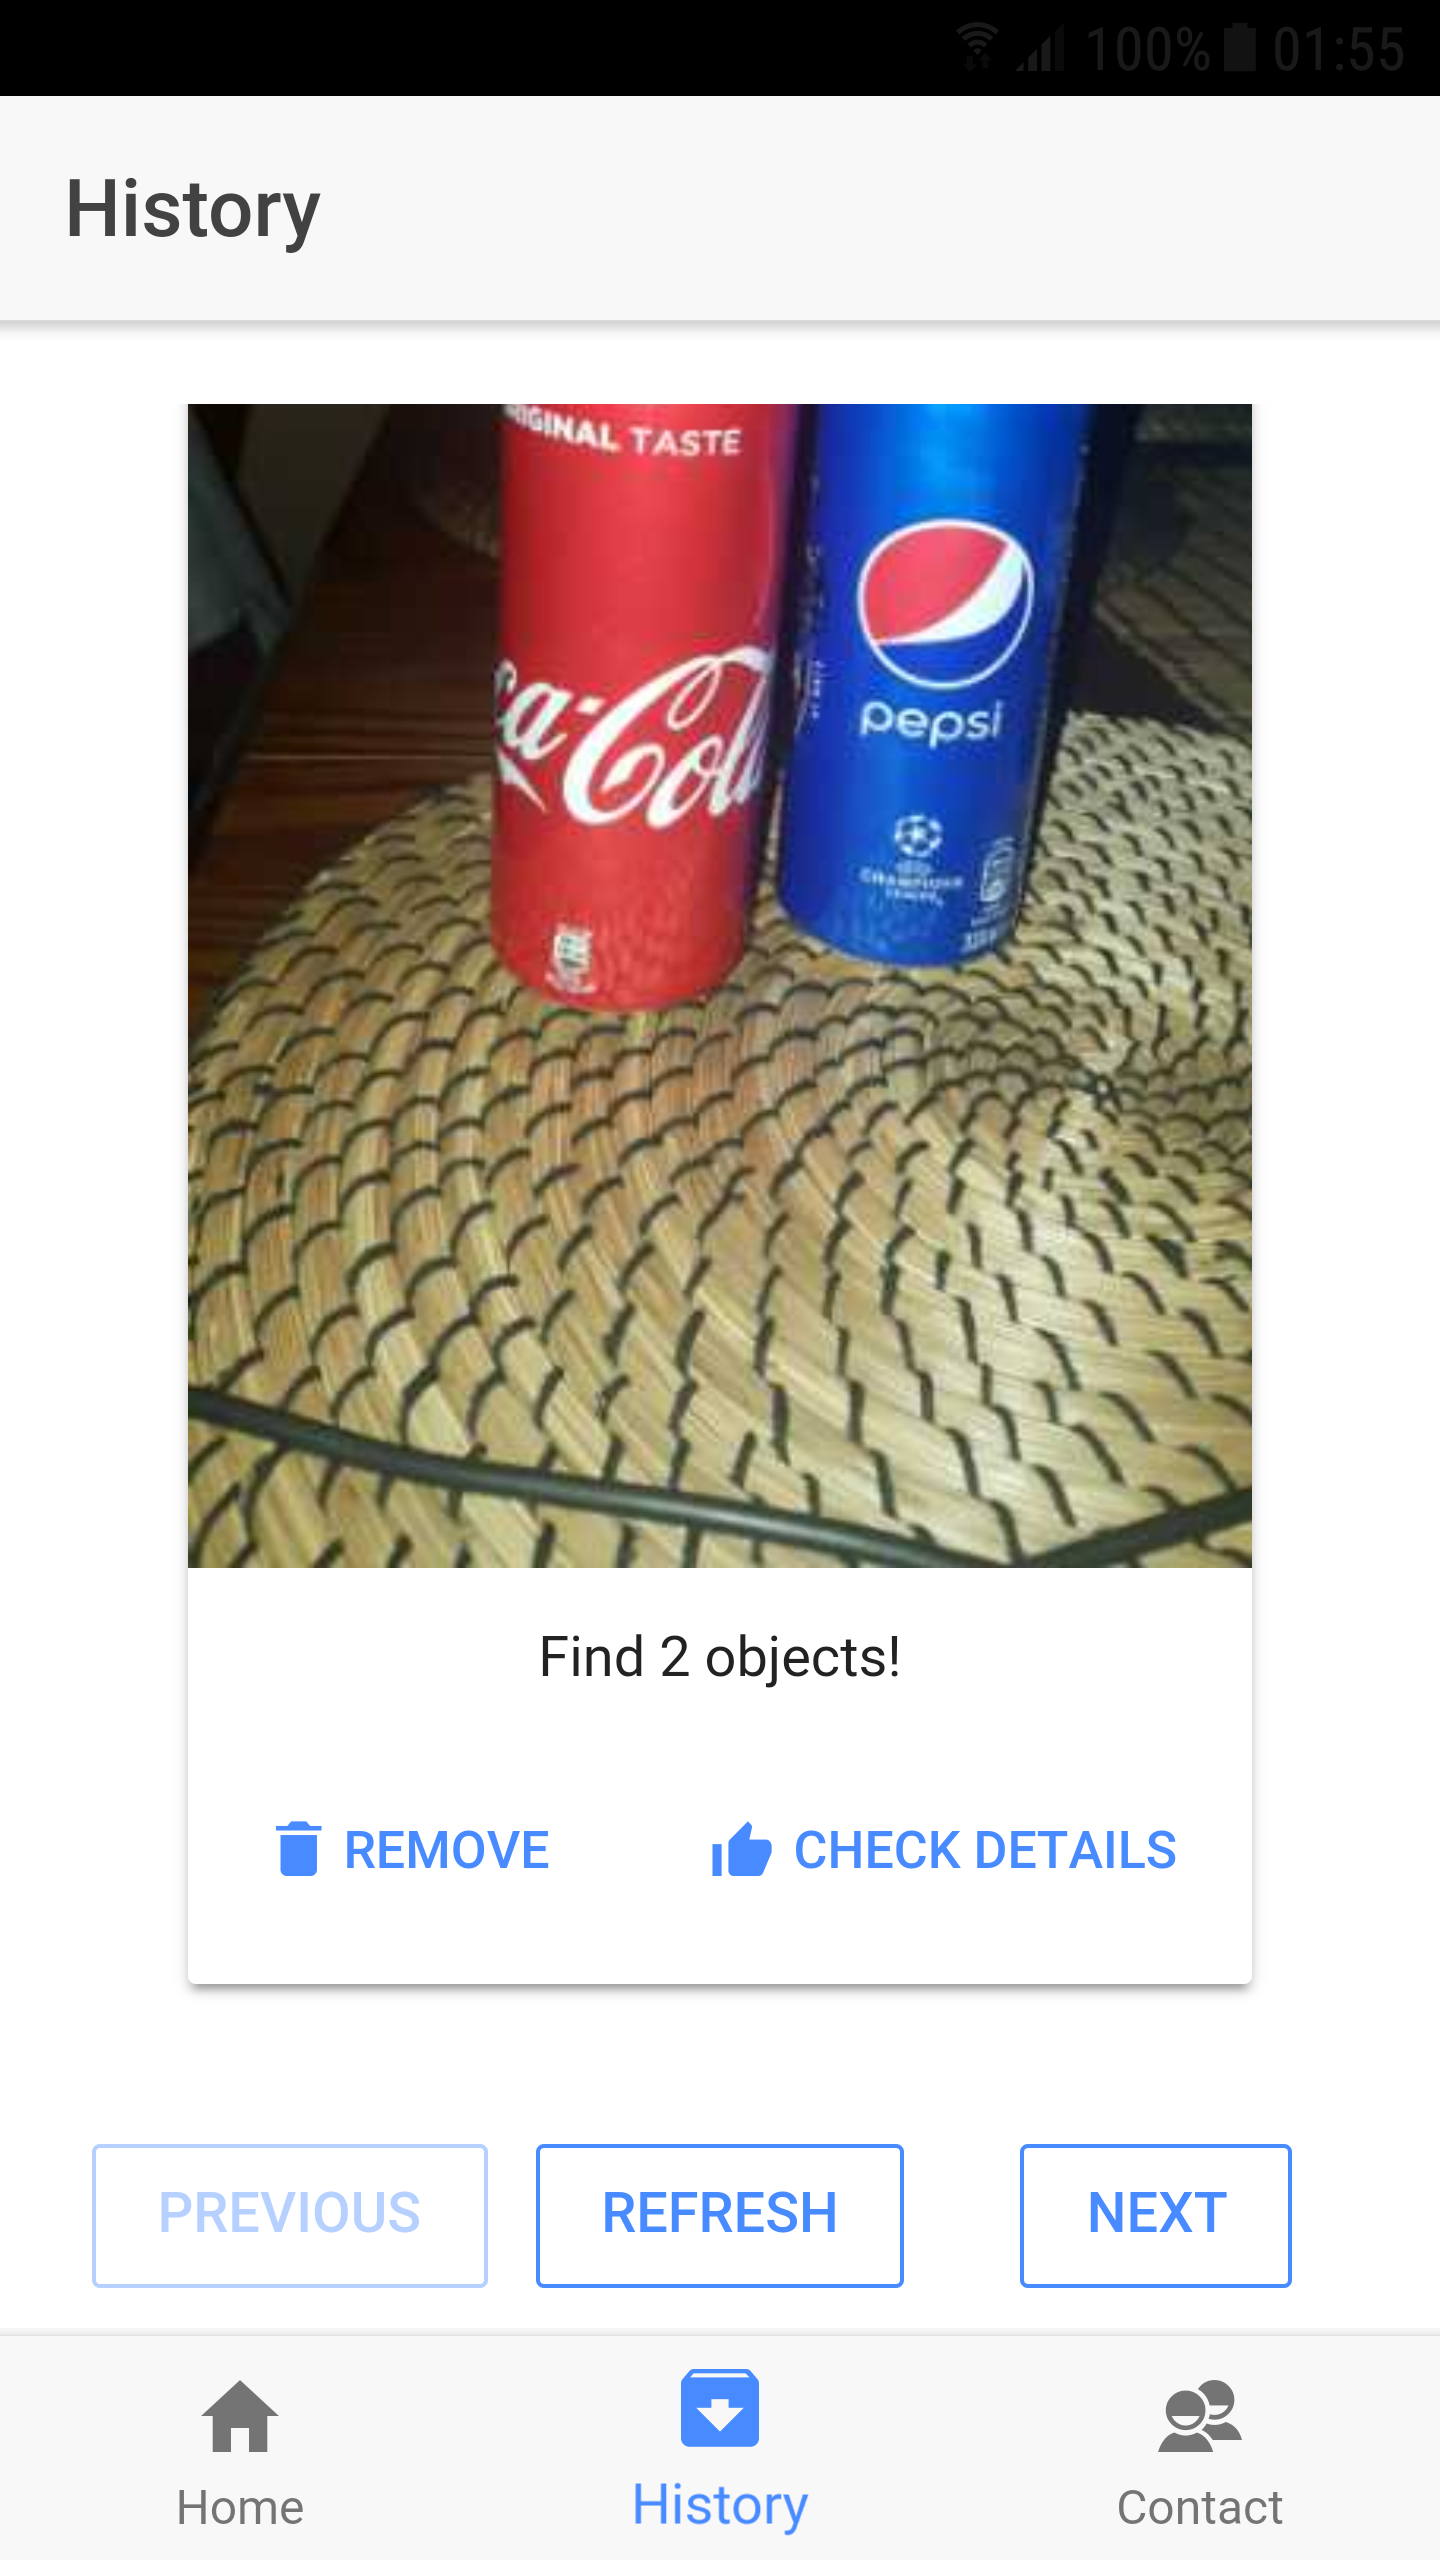
\includegraphics[width=0.4\textwidth]{images/history list}}
	\caption{Ekran szczegółów analizowanego zdjęcia oraz historia.}
	\label{fig:uploadView}
\end{figure}

Użytkownik z ekranu głównego aplikacji ma dostęp do zakładki kontakt. Zostały w niej zostały informacje o autorze aplikacji.



